\section{Evaluación}

\subsection{Test enron}

La primera clasificación requerida, que hemos denominado directamente ``enron'',
consiste en una division por carpetas de la base de correos. El conjunto de
entrenamiento consiste en todos los correos de las carpetas enron1 a enron5, y
el conjunto de evaluación está compuesto por la carpeta restante, enron6.  Se ha
realizado un test utilizando un umbral de probabilidad de 0.5 y la estrategia de
tokenización ``basic''. La matriz de confusión obtenida se muestra a
continuación.

\begin{table}[ht]
	\centering
	\begin{tabular}{l|l|l|}
	\cline{2-3}
				   & Ham     & Spam    \\ \hline
	\multicolumn{1}{|l|}{Ham}  & 24.75\% & 0.25\%  \\ \hline
	\multicolumn{1}{|l|}{Spam} & 5.92\%  & 69.08\% \\ \hline
	\end{tabular}
	\caption{Matriz de confusión del test de enron}
	\label{tab:test-enron}
\end{table}

El sistema ha sido capaz de clasificar correctamente un 93.83\% de los correos.
Observando el conjunto de correos que no han sido clasificados correctamente, se
pueden encontrar, entre otros, correos muy cortos y correos con una redacción
muy característica de correos tipo ham.

\clearpage
\subsection{Test 75\% entrenamiento, 25\% evaluación}

La segunda clasificación requerida consiste en dividir aleatoriamente la base de
correos, usando un 75\% para entrenamiento y un 25\% para evaluación.

\begin{figure}[ht]
	\centering
	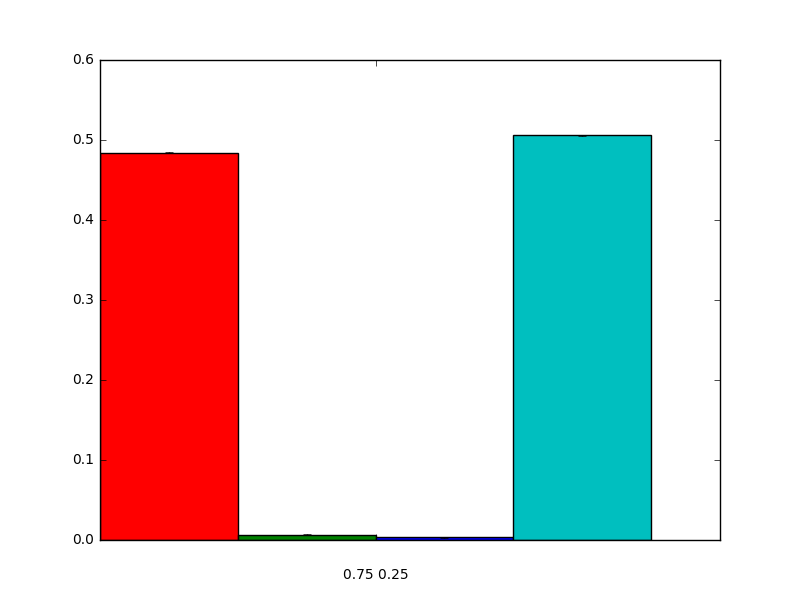
\includegraphics[width=\textwidth, keepaspectratio]{img/7525}
	\caption{Resultados del test 75\%-25\%}
	\label{fig:7525}
\end{figure}

El resultado obtenido es muy similar al test ``enron'', con un alto porcentaje
de correos clasificados satisfactoriamente. La gráfica muestra la media y
desviación típica de las pruebas, siendo ésta última prácticamente nula.

\clearpage
\subsection{Test [0.05-50]\% entrenamiento, 20\% evaluación}

El siguiente test ha sido realizado con un 20\% de correos para evaluación, y un
conjunto variable entre 0.05\% y 50\% para el conjunto de entrenamiento.

\begin{figure}[ht]
	\centering
	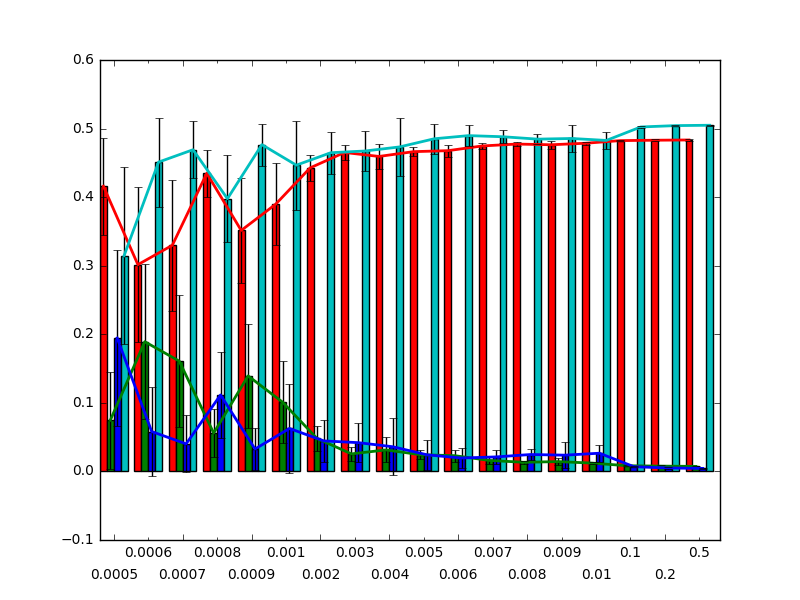
\includegraphics[width=\textwidth, keepaspectratio]{img/ev_tr}
	\caption{Resultados del test [0.05-50]\%-20\%}
	\label{fig:ev_tr}
\end{figure}

Se puede observar que para un tamaño muy pequeño del conjunto de entrenamiento,
el sistema clasifica los correos de una forma menos satisfactoria que en las
pruebas anteriores, y que ademas hay mucha desviación típica en los tests. Al
aumentar el tamaño del conjunto de entrenamiento, aumenta la precisión del
sistema de manera rápida y se consigue una saturación en su rendimiento. Esto
puede ser debido a que la base de correos contiene mayormente correos con
características muy similares.

\clearpage
\subsection{Test umbral}

Este test se ha realizado variando el umbral a partir del cual un correo es
considerado spam.

Con un umbral muy bajo el sistema consigue una cantidad relativamente elevada
de falsos positivos, la cual disminuye rápidamente al aumentar el umbral, a la
vez que aumenta la cantidad de correos de ham clasificados correctamente. La
cantidad de correos de spam clasificados correctamente se mantiene estable en
casi todo el rango, salvo en valores altos del umbral, donde le ocurre lo mismo
que a la clasificación de correos de ham en valores bajos. Esto es indicativo
de que existen muchos correos que generan unos valores de probabilidad muy
cercanos a 0 o a 1, los cuales son muy fáciles de clasificar por el algoritmo.
Además, existe un número menor de ellos que consiguen probabilidades mejor
distribuidas en el intervalo $[0,1]$, que son más difíciles de clasificar.

\begin{figure}[hb]
	\centering
	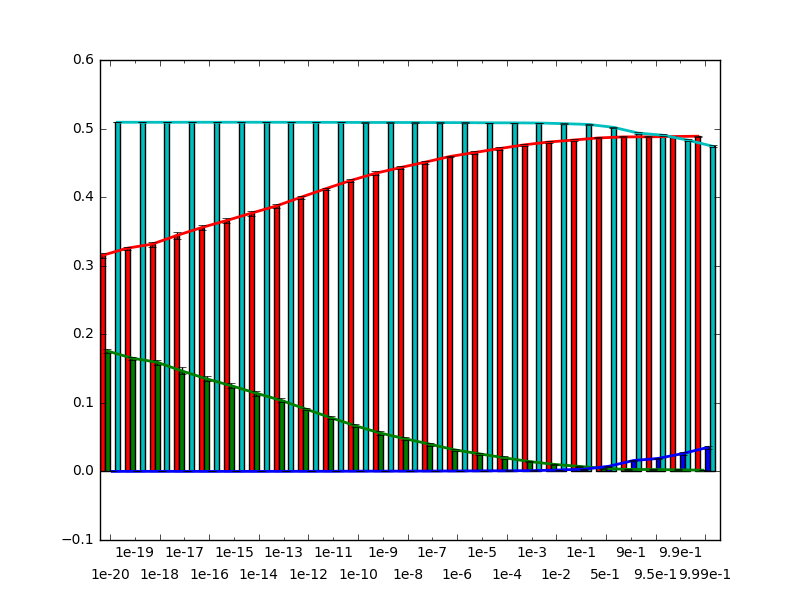
\includegraphics[width=\textwidth, keepaspectratio]{img/threshold}
	\caption{Resultados del tests de umbral, parte de spam (variando entre
	1e-20 hasta 0.999)}
	\label{fig:threshold}
\end{figure}

\begin{figure}[hb]
	\centering
	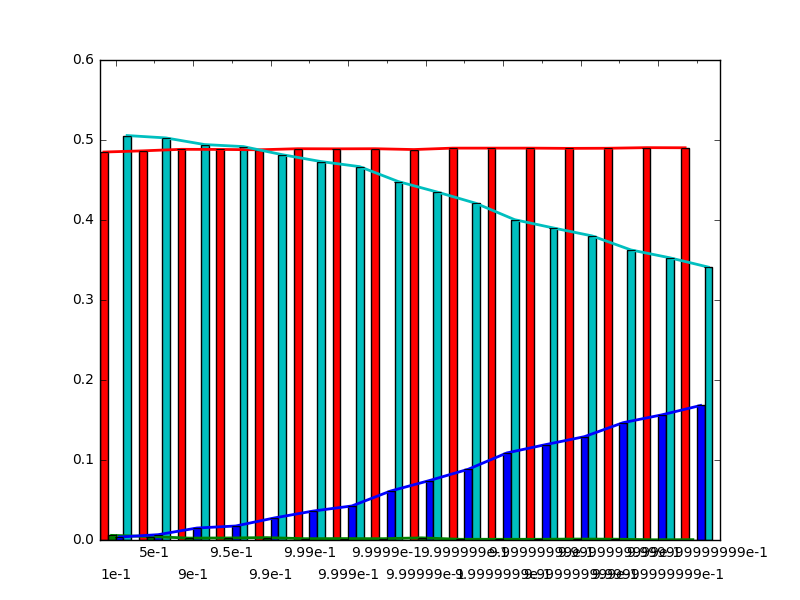
\includegraphics[width=\textwidth, keepaspectratio]{img/threshold2}
	\caption{Resultados del tests de umbral, parte de ham (variando entre
	1e-2 hasta 0.9999999999999)}
	\label{fig:threshold2}
\end{figure}

\clearpage
\subsection{Test estrategias de tokenización}

Este test prueba las diferentes estrategias de división de un correo en tokens.

\begin{figure}[ht]
	\centering
	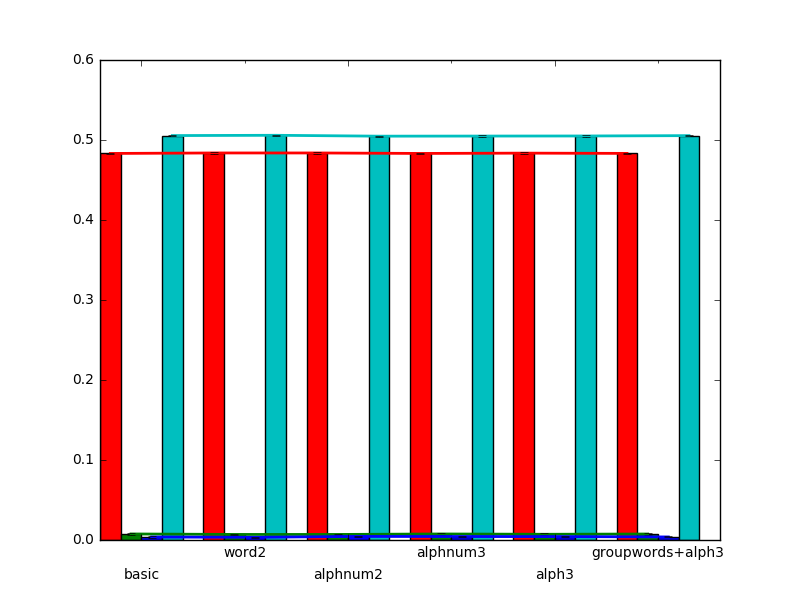
\includegraphics[width=\textwidth, keepaspectratio]{img/tokens}
	\caption{Resultados del test de estrategias de tokenización}
	\label{fig:tokens}
\end{figure}

La calidad de la clasificación es prácticamente la misma en todas las
estrategias. Esto puede ser debido a que la funcionalidad de la estrategia más
básica, ``basic'', está esencialmente contenida dentro de las demás, y parece
ser suficiente para la correcta clasificación de la base de correos.
